
\textbf{Pour cette première partie, aucune justification n'est demandée et une seule réponse est possible par question. Pour chaque question, reportez son numéro sur votre copie et indiquez votre réponse.}

\subsubsection*{Question 1}

\begin{minipage}[t]{0.5\textwidth}
On considère l'arbre de probabilité ci-contre.

On cherche la probabilité de l'évènement B.

\medskip

On a
\end{minipage}
%\hfill
\begin{minipage}[t]{0.45\textwidth}
\vspace{0pt}
\begin{center}
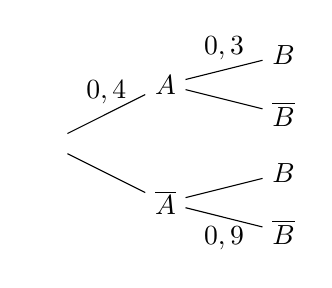
\begin{tikzpicture}[scale=0.75]
\node (P_-1_0) at (-2,-1.5) {$\phantom{A}$};
\node (P_0_0) at (0,-0.5) {$A$};
\draw (P_-1_0) -- (P_0_0) node[midway, above] {$0,4$};
\node (P_1_0) at (2,-0) {$B$};
\draw (P_0_0) -- (P_1_0) node[midway, above] {$0,3$};
\node (P_1_1) at (2,-1) {$\overline{B}$};
\draw (P_0_0) -- (P_1_1) node[midway, below] {};
\node (P_0_2) at (0,-2.5) {$\overline{A}$};
\draw (P_-1_0) -- (P_0_2) node[midway, below] {};
\node (P_1_2) at (2,-2) {$B$};
\draw (P_0_2) -- (P_1_2) node[midway, above] {};
\node (P_1_3) at (2,-3) {$\overline{B}$};
\draw (P_0_2) -- (P_1_3) node[midway, below] {$0,9$};
\end{tikzpicture}
\end{center}
\end{minipage}

\textbf{a.} $p(B) = 0,18$\hfill \textbf{b.} $p(B) = 0,12$\hfill \textbf{c.} $p(B) = 0,66$\hfill \textbf{d.} $p(B) = 0,3$

\subsubsection*{Question 2}
Une tablette coûte 200 euros. Son prix diminue de 30\%. Le prix après cette diminution est :

\textbf{a.} 140 euros\hfill \textbf{b.} 170 euros\hfill \textbf{c.} 194 euros\hfill \textbf{d.} 197 euros

\subsubsection*{Question 3}
Une réduction de 50\% suivie d'une augmentation de 50\% équivaut à :

\textbf{a.} une réduction de 50\%\hfill \textbf{b.} une réduction de 25\%

\textbf{c.} une augmentation de 25\%\hfill \textbf{d.} une augmentation de 75\%

\subsubsection*{Question 4}
Dans un lycée, le quart des élèves sont internes, parmi eux, la moitié sont des filles.

La proportion des filles internes par rapport à l'ensemble des élèves du lycée est égale à :

\textbf{a.} 4\%\hfill \textbf{b.} 12,5\%\hfill \textbf{c.} 25\%\hfill \textbf{d.} 50\%

\subsubsection*{Question 5}
On considère le nombre $N = \dfrac{10^7}{5^2}$. On a :

\textbf{a.} $N = 2^5$\hfill \textbf{b.} $N = 20\,000$\hfill \textbf{c.} $N = \dfrac{1}{10^5}$\hfill \textbf{d.} $N = 4 \times 10^5$

\subsubsection*{Question 6}
Un appareil a besoin d'une énergie de $7,5 \times 10^6$ Joules (J) pour se mettre en route.

À combien de kiloWatts-heure (kWh) cela correspond-il ?

\begin{flushright}
\uline{\textit{Données}} : 1kWh = $3,6 \times 10^6$ J.
\end{flushright}

\textbf{a.} $0,5$ kWh\hfill \textbf{b.} $2,08$ kWh\hfill \textbf{c.} $5,3$ kWh\hfill \textbf{d.} $20,35$ kWh

\subsubsection*{Question 7}
Le plan est muni d'un repère orthogonal. On note $d$ la droite passant par les points A$(0~;~-1)$ et B$(2~;~5)$. Le coefficient directeur de la droite $d$ est égal à :

\textbf{a.} $-\dfrac{1}{2}$\hfill \textbf{b.} $2$\hfill \textbf{c.} $3$\hfill \textbf{d.} $\dfrac{1}{3}$

\bigskip

\begin{minipage}[t]{0.8\textwidth}
\subsubsection*{Question 8}
On a représenté ci-contre une droite $D$.

Parmi les quatre équations ci-dessous, la seule susceptible de représenter la droite $D$ est :

\textbf{a.} $2x - y = 0$\hfill \textbf{b.} $2x + y + 1 = 0$

\textbf{c.} $y = x^2 - (x + 1)^2 + 1$\hfill \textbf{d.} $y = 2x - 1$
\end{minipage}
\hfill
\begin{minipage}[t]{0.15\textwidth}
\vspace{0pt}
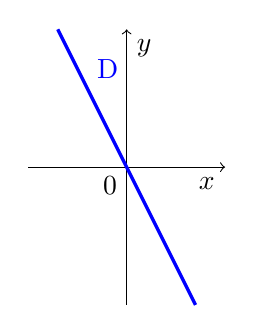
\begin{tikzpicture}[scale=0.5]
    \draw[->] (-2.5,0) -- (2.5,0) node[thick, below left]{$x$};
    \draw[->] (0,-3.5) -- (0,3.5) node[thick, below right]{$y$};
    \node[below left] at (0,0) {0};
    \draw[domain=-1.75:1.75, smooth, variable=\x, blue, very thick] plot ({\x}, {-2*\x});
    \node[above right, blue] at (-1, 2) {D};
\end{tikzpicture}
\end{minipage}

\subsubsection*{Question 9}
On note $S$ l'ensemble des solutions de l'équation $x^2 = 10$ sur $\R$. On a :

\textbf{a.} $S = \{-5~;~5\}$\hfill \textbf{b.} $S = \{-\sqrt{5}~;~\sqrt{5}\}$

\textbf{c.} $S = \{-\sqrt{10}~;~\sqrt{10}\}$\hfill \textbf{d.} $S = \emptyset$

\subsubsection*{Question 10}
La fonction $f$ définie sur $\R$ par $f(x) = (3x - 15)(x + 2)$ admet pour tableau de signes :

\textbf{a.} 
\begin{tabular}{|c|ccccccc|}
\hline
$x$ & $-\infty$ & & $-2$ & & $5$ & & $+\infty$ \\
\hline
$f(x)$ & & $+$ & $0$ & $-$ & $0$ & $+$ &\\
\hline
\end{tabular}
\hfill 
\textbf{b.} 
\begin{tabular}{|c|ccccccc|}
\hline
$x$ & $-\infty$ & & $-2$ & & $5$ & & $+\infty$ \\
\hline
$f(x)$ & & $-$ & $0$ & $+$ & $0$ & $-$ &\\
\hline
\end{tabular}

\textbf{c.} 
\begin{tabular}{|c|ccccccc|}
\hline
$x$ & $-\infty$ & & $-5$ & & $2$ & & $+\infty$ \\
\hline
$f(x)$ & & $+$ & $0$ & $-$ & $0$ & $+$ &\\
\hline
\end{tabular}
\hfill 
\textbf{d.} 
\begin{tabular}{|c|ccccccc|}
\hline
$x$ & $-\infty$ & & $-5$ & & $2$ & & $+\infty$ \\
\hline
$f(x)$ & & $-$ & $0$ & $+$ & $0$ & $-$ &\\
\hline
\end{tabular}

\subsubsection*{Question 11}
L'expression développée de $(2x + 0,5)^2$ est :

\textbf{a.} $4x^2 + x + 0,25$\hfill \textbf{b.} $4x^2 + 4x + 2$

\textbf{c.} $4x^2 + 2x + 0,25$\hfill \textbf{d.} $4x^2 + 2x + 1$

\subsubsection*{Question 12}
Lorsqu'un point mobile suit une trajectoire circulaire de rayon $R$, en mètre (m), son accélération centripète $a$ (en m/s$^2$) s'exprime en fonction de la vitesse $v$ (en m/s) de la manière suivante :

\[a = \dfrac{v^2}{R}\]

L'expression permettant, à partir de cette formule, d'exprimer la vitesse $v$ est :

\textbf{a.} $v = aR^2$\hfill \textbf{b.} $v = \sqrt{aR}$

\textbf{c.} $v = \sqrt{\dfrac{a}{R}}$\hfill \textbf{d.} $v = \dfrac{a^2}{R}$




\begin{center}
\textbf{\large DEUXIÈME PARTIE (14 pts)}
\end{center}

